\documentclass{standalone}
\usepackage{amsmath,amssymb,pgfmath,pgffor,tikz,xcolor,xifthen}
\usetikzlibrary{calc,decorations.pathmorphing,decorations.pathreplacing,patterns,backgrounds}


\begin{document}

% \def\x{20}
% \def\xx{27}
% \def\y{9}
% \def\d{4}
% \def\a{1}
% \def\b{4}
% \def\c{1}
% \def\e{0.75}
% \def\f{3}
% \def\g{2}

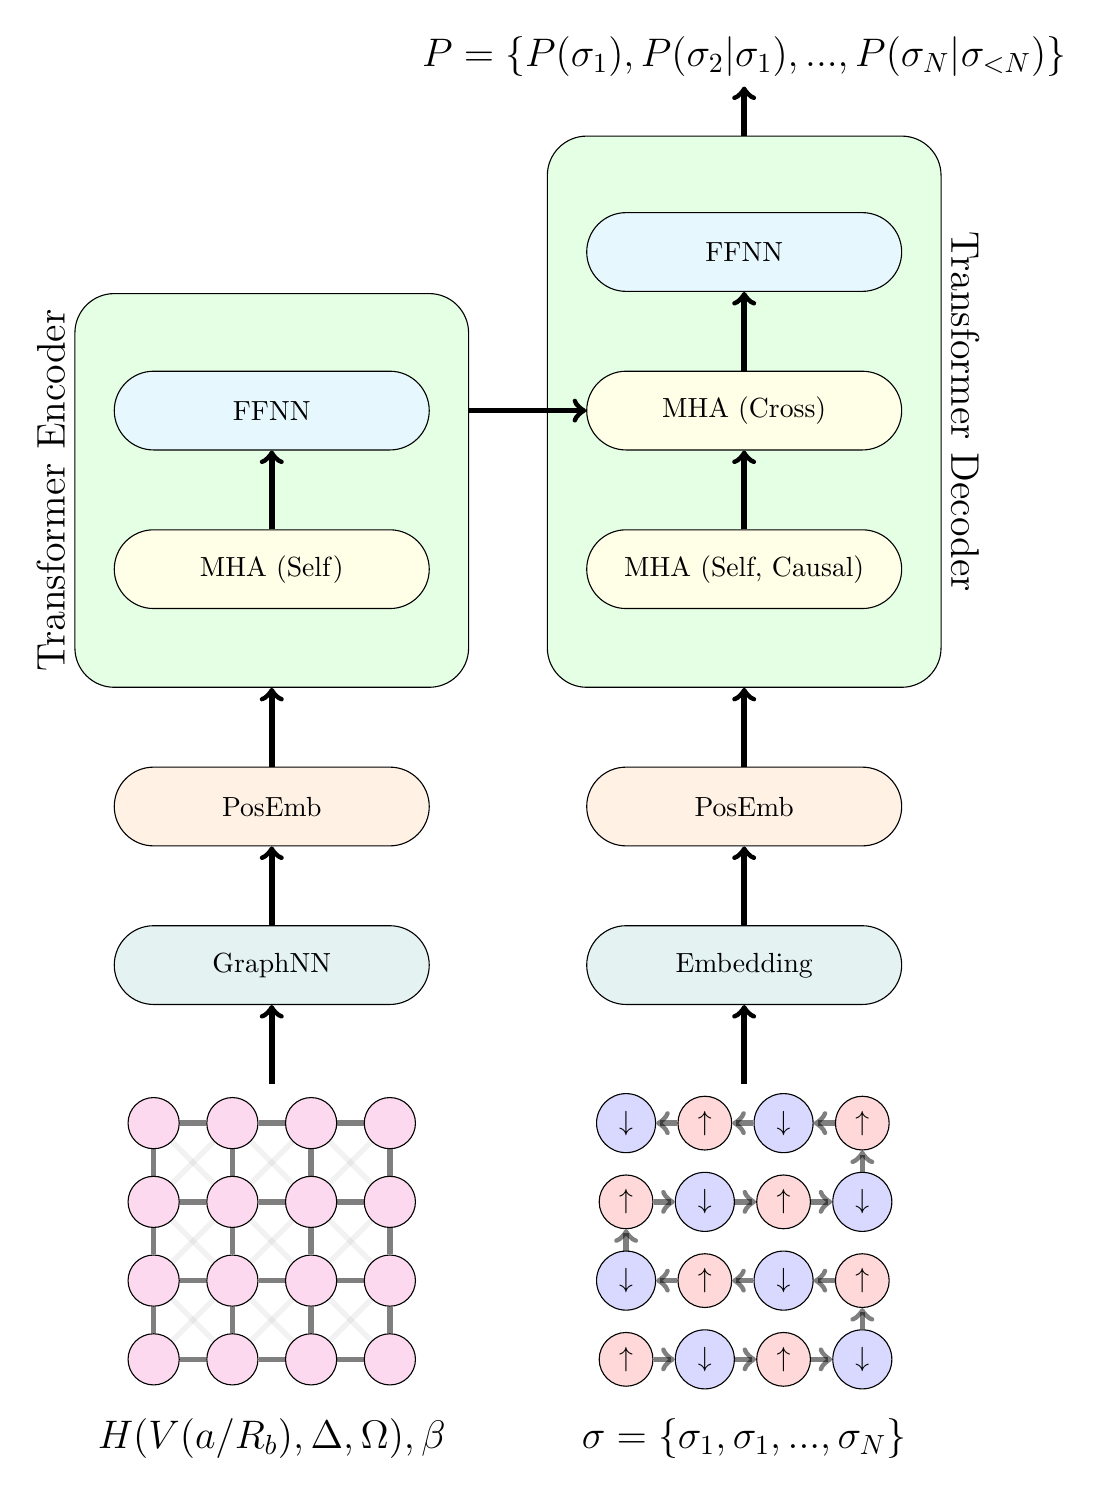
\begin{tikzpicture}

\def\L{4}
\def\Lm{3}
\foreach \i in {1,...,\L} {
\foreach \j in {1,...,\L} {
    \node [circle,fill=magenta!15,draw,minimum size=0.65cm] (spin-\i-\j) at ($(\i,\j) + (0,0)$) {};
}
}

\foreach \i in {1,...,\Lm} {
\foreach \j in {1,...,\L} {
    \pgfmathsetmacro\ip{int(\i+1)}
    \pgfmathsetmacro\jp{int(\j+1)}
    \draw [-, opacity=0.5, line width = 2] (spin-\i-\j) -- (spin-\ip-\j);
}
}

\foreach \i in {1,...,\L} {
\foreach \j in {1,...,\Lm} {
    \pgfmathsetmacro\ip{int(\i+1)}
    \pgfmathsetmacro\jp{int(\j+1)}
    \draw [-, opacity=0.5, line width = 2] (spin-\i-\j) -- (spin-\i-\jp);
}
}

\foreach \i in {1,...,\Lm} {
\foreach \j in {1,...,\Lm} {
    \pgfmathsetmacro\ip{int(\i+1)}
    \pgfmathsetmacro\jp{int(\j+1)}
    \draw [-, opacity=0.05, line width = 2] (spin-\i-\j) -- (spin-\ip-\jp);
}
}

\foreach \i in {1,...,\Lm} {
\foreach \j in {2,...,\L} {
    \pgfmathsetmacro\ip{int(\i+1)}
    \pgfmathsetmacro\jm{int(\j-1)}
    \draw [-, opacity=0.05, line width=2] (spin-\i-\j) --  (spin-\ip-\jm);
}
}

\node [align=center] at (\L/2+0.5, 0 ) {\Large $H(V(a / R_b), \Delta, \Omega), \beta$};

\coordinate (input1) at (\L/2+0.5,\L+0.5) ;

\node [align=center,anchor=south, rectangle, fill=teal!10, draw, rounded corners=0.5cm, minimum height=1cm, minimum width=4cm] (enc_graphnn) at ($(input1.north) + (0,1)$) {GraphNN};

\node [align=center,anchor=south, rectangle, fill=orange!10, draw, rounded corners=0.5cm, minimum height=1cm, minimum width=4cm] (enc_posemb1) at ($(enc_graphnn.north) + (0,1)$) {PosEmb};

\node [align=center,anchor=south, rectangle, fill=green!10, draw, rounded corners=0.5cm, minimum height=5cm, minimum width=5cm] (tfenc) at ($(enc_posemb1.north) + (0,1)$) {};
\node [anchor=east] at (tfenc.west) {\Large \rotatebox{90}{Transformer Encoder}};

\node [align=center,anchor=south, rectangle, fill=yellow!10, draw, rounded corners=0.5cm, minimum height=1cm, minimum width=4cm] (enc_mha_self) at ($(tfenc.south) + (0,1)$) {MHA (Self)};
\node [align=center,anchor=south, rectangle, fill=cyan!10, draw, rounded corners=0.5cm, minimum height=1cm, minimum width=4cm] (enc_ffnn) at ($(enc_mha_self.north) + (0,1)$) {FFNN};

\draw [->,line width=2] (input1) -- (enc_graphnn);
\draw [->,line width=2] (enc_graphnn) -- (enc_posemb1);
\draw [->,line width=2] (enc_posemb1) -- (tfenc);
\draw [->,line width=2] (enc_mha_self) -- (enc_ffnn);

%%%%%%%%%%%%%%%%%%%%%%%%%%%%%%%%%%%%%%%%%%%%%%%%%%%%%%%%%%%%%%%%%%%%%%%%%%%%%%%%%%%%%%%%

\foreach \i in {1,...,\L} {
\foreach \j in {1,...,\L} {
    \pgfmathsetmacro\k{int(\i+\L*(\j-1))}
    \pgfmathsetmacro\m{mod(\i+\j,2)}
    \ifthenelse{\equal{\m}{0.0}}{
    \node [circle,fill=red!15,draw,minimum size=0.65cm] (spin2-\i-\j) at ($(\i,\j) + (6,0)$) {$\uparrow$};
    }
    {
    \node [circle,fill=blue!15,draw,minimum size=0.75cm] (spin2-\i-\j) at ($(\i,\j) + (6,0)$) {$\downarrow$};
    }
}
}

\foreach \i in {1,...,\Lm} {
\foreach \j in {1,...,\L} {
    \pgfmathsetmacro\ip{int(\i+1)}
    \pgfmathsetmacro\jp{int(\j+1)}
    \pgfmathsetmacro\k{mod(\j,2)}
    \ifthenelse{\equal{\k}{1.0}}{
    \draw [->, opacity=0.5, line width = 2] (spin2-\i-\j) -- (spin2-\ip-\j);
    }
    {
    \draw [<-, opacity=0.5, line width = 2] (spin2-\i-\j) -- (spin2-\ip-\j);
    }
}
}

\foreach \j in {1,...,\Lm} {
    \pgfmathsetmacro\jp{int(\j+1)}
    \pgfmathsetmacro\ip{int(1 + mod(\j,2)*\Lm)}
    \draw [->, opacity=0.5, line width = 2] (spin2-\ip-\j) -- (spin2-\ip-\jp);
}

\node [align=center] at ($(\L/2+0.5, 0) + (6,0)$) {\Large $\sigma = \{ \sigma_1,\sigma_1,...,\sigma_N \}$};

\coordinate (input2) at ($(input1) + (6,0)$);

\node [align=center,anchor=south, rectangle, fill=teal!10, draw, rounded corners=0.5cm, minimum height=1cm, minimum width=4cm] (dec_emb) at ($(input2.north) + (0,1)$) {Embedding};

\node [align=center,anchor=south, rectangle, fill=orange!10, draw, rounded corners=0.5cm, minimum height=1cm, minimum width=4cm] (dec_posemb) at ($(dec_emb.north) + (0,1)$) {PosEmb};

\node [align=center,anchor=south, rectangle, fill=green!10, draw, rounded corners=0.5cm, minimum height=7cm, minimum width=5cm] (tfdec) at ($(dec_posemb.north) + (0,1)$) {};
\node [anchor=west] at (tfdec.east) {\Large \rotatebox{270}{Transformer Decoder}};

\node [align=center,anchor=south, rectangle, fill=yellow!10, draw, rounded corners=0.5cm, minimum height=1cm, minimum width=4cm] (dec_mha_selfcausal) at ($(tfdec.south) + (0,1)$) {MHA (Self, Causal)};
\node [align=center,anchor=south, rectangle, fill=yellow!10, draw, rounded corners=0.5cm, minimum height=1cm, minimum width=4cm] (dec_mha_cross) at ($(dec_mha_selfcausal.north) + (0,1)$) {MHA (Cross)};
\node [align=center,anchor=south, rectangle, fill=cyan!10, draw, rounded corners=0.5cm, minimum height=1cm, minimum width=4cm] (dec_ffnn) at ($(dec_mha_cross.north) + (0,1)$) {FFNN};


\node (output2) at($(tfdec.north) + (0,1)$) {\Large $P = \{ P(\sigma_1), P(\sigma_2|\sigma_1),...,P(\sigma_N|\sigma_{<N}) \}$};

\draw [->,line width=2] (input2) -- (dec_emb);
\draw [->,line width=2] (dec_emb) -- (dec_posemb);
\draw [->,line width=2] (dec_posemb) -- (tfdec);
\draw [->,line width=2] (tfdec) -- (output2);
\draw [->,line width=2] (dec_mha_selfcausal) -- (dec_mha_cross);
\draw [->,line width=2] (dec_mha_cross) -- (dec_ffnn);
\draw [->,line width=2] (tfenc.east |- dec_mha_cross.west) -- (dec_mha_cross.west);


\end{tikzpicture}

\end{document}
